\section{Results}

The first capability of the introduced system to proof is 
to solve complex interactions and iterations loops that are of a non-linear kind.
Therefor a material hoists is chosen, 
due to the fact that the motor weight adds 
to the overall weight of the lift (fig. \ref{pic:lift_model}), 
hence causing a simple iteration loop.
With current methods eigenweight problems in the part design are often simplfied 
by over estimating the total load on the motor.
This over estimation garants a safty tolerance.
In cases where mass reduction is crutial like in aircraft and space applications, this is often not an option.
\begin{figure}[h]
    \centering
    \begin{subfigure}[b]{0.55\textwidth}
        \centering
        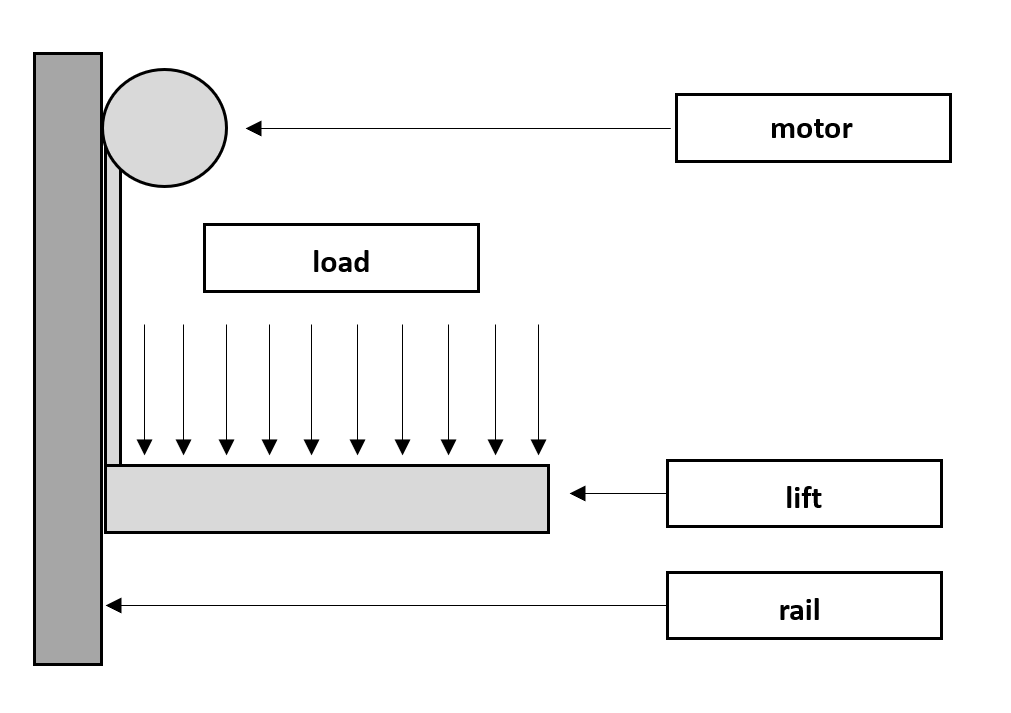
\includegraphics[width=\textwidth]{pics/500Z_model.png}
        \caption{\label{pic:lift_model} Model of a material lift.}
    \end{subfigure}
    \hfill
    \begin{subfigure}[b]{0.95\textwidth}
        \centering
        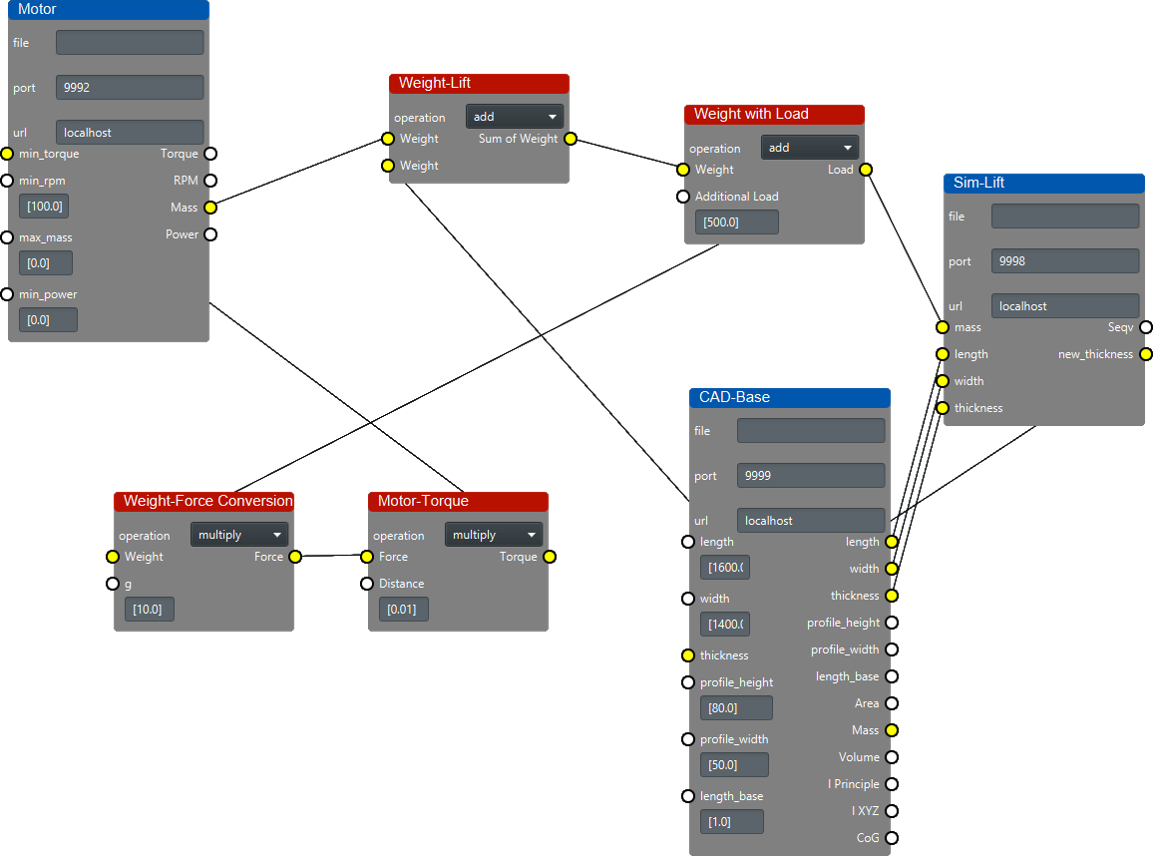
\includegraphics[width=\textwidth]{pics/500Z_solution.png}
        \caption{\label{pic:lift_solu} Implementation of the design process.}
    \end{subfigure}
    \caption{\label{pic:lift} Designing of a material lift with the introduced framework.}
\end{figure}\\
Modelling the complex interaction of the hoist parts with the developed software allows to automatically update, change and test the current configuration.
Therefor the simplified model is broken into several process, each describing the individual parts and their influence on different parameters of the hoist (fig. \ref{pic:lift_solu}).\\
The motor process in figure \ref{pic:lift} represents the selection process of a new motor, based on the minimum torque, RPM, power or maximum mass.
Realistically, determining the motor properties would be done by searching in a database, but open motor databases have many restrictions.
Therefor this program calculates a motor based on a simple motor model.\\
The base of the hosit is represented by two systems:
The CAD-Base cahnges a simplified CAD model (fig. \ref{pic:lift}).
The generated file is then  transfered to the simulation process.
There the inserted loads are applied to the model and the relevant stresses are outputed.\\
Against the usual material hosits with a high tolerance for failure,
the system is with safety factor of 1.2 more on the lightweight spectrum.
The developed system needed, depending on the intitial configuration, up to 12 iteration (each iteration needs about 1 min to fully compute on a normal laptop) to find the solution.
Designing a system with a eigenweight problem and a small safety nomaly takes a long time.
Hence it is difficult to find suitable refernce data, the follwing assumtion can be made.
By assuming that each step takes 30 min per iterations, solving the same problem by hand would take up to 6h instead of 12 min by the program.\\
But the seen time savings have to be taken with care.
In the proposed problem it is assumed that both, manual and automated solutions uses the same infrastructure of pre-build simulations, constructions, etc. that are not taking into the overal time.
Further, the automated process uses data interfaces to reuse the CAD-model in the simulation process.
Other usecases might require costom conversion and representations interfaces, hence increasing the setup time of such a system.\\
The material lift is not suited to show a complex optimization problem.
Thats why a further use cases is introduced, 
in which an optimal layer composition of a 
high-speed glass fiber composite(GFC)-rotor has to be determined (fig. \ref{pic:rotor_model}).
High-speed composite rotors undergo inhomogeneous and variable stress states induced
by centrifugal forces, which are mainly characterised by multi-axial tension and shear
loads, \cite{filippatos_damage_2017}.
The observed damage behavior is closely joint with the composition of the fibre-matrix, 
what increases the structural complexity.
Furthermore, compression loads can be caused by impact loads leading to inter-fibre failure and delaminations.
The dynamic response of rotors is further affected by the apparent stiffening from
the applied centrifugal forces. 
Consequently, the analysis and description of the damage
and dynamic behavior usually requires more complex approaches for high-speed composite
rotors than for similar stationary structures \cite{filippatos_damage_2017}.\\
The interaction of load induced structural and damage behavior, lead to many opportunities for different optimization approaches. 
This example is designed to show and validate the optimization of to properties which negate each other.
Therefore, the rotor will be designed to sustain a certain angular velocity, while not starting to vibrate to the rotor oscillation.
The rotor is a simple disk with an outer and inner diameter, a constant height.
In this use case the rotor should, similar to \cite{Filippatos2021}, consist of only unsymmetrically layer compositions.
Each layer consists of unidirectional GFK-fiber material,
which can be oriented in radial or tangent direction.
Further, it is assumed that the material will instantly break if the first principle stress reach a the point of rupture.
\begin{figure}[h]
    \centering
    \begin{subfigure}[b]{0.95\textwidth}
        \centering
        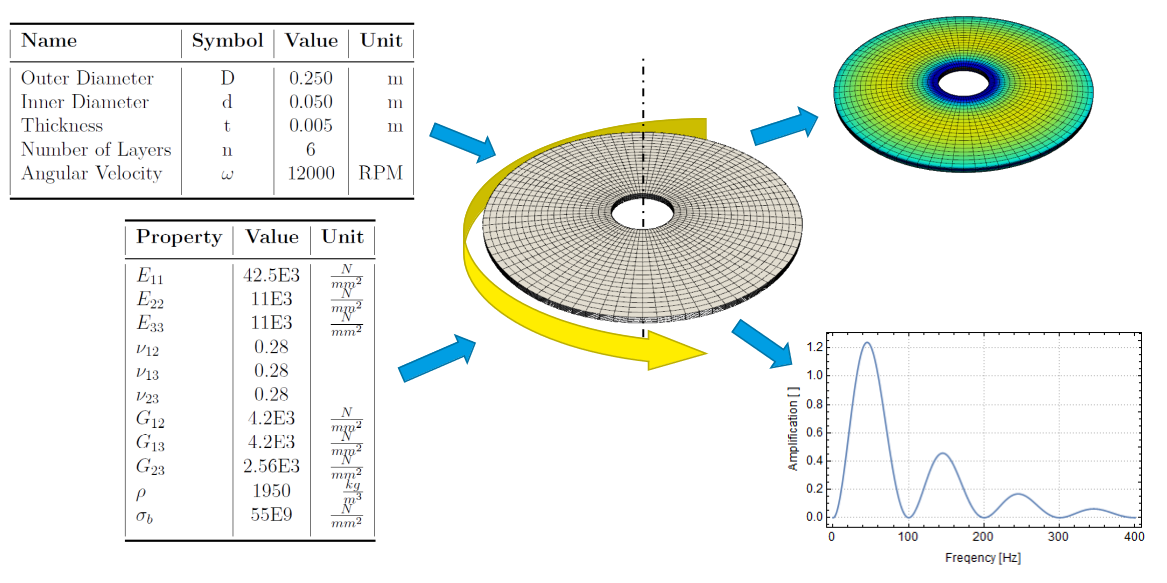
\includegraphics[width=\textwidth]{pics/rotor_model.png}
        \caption{\label{pic:rotor_model} Model of a material lift.}
    \end{subfigure}
    \hfill
    \begin{subfigure}[b]{0.95\textwidth}
        \centering
        \includegraphics[width=\textwidth]{pics/rotor_solution.png}
        \caption{\label{pic:rotor_solution} Implementation of the design process.}
    \end{subfigure}
    \caption{\label{pic:rotor} Designing of a material lift with the introduced framework.}
\end{figure}\\
Simulating the development process in the developed software is done by 
modelling the material and the rest of the rotor separately, as shown in figure \ref{pic:rotor_solution}.
This modular approach enables to quickly change the material properties and to reuse the material database.
it further allows to switch easily between different materials and combinations.\\
The generated solutions are grouped as follwing:
\begin{enumerate}
    \item suitable solutions (principle stress below rupture stress)
    \item unsuitable solutions (principle stress over rupture stress)
\end{enumerate}
From these two groups only the first suitable solutions are used further.
A fitness value is then computed based on a function which represents the following rules to describe an optimal solution:
\begin{enumerate}
    \item the amount of the principle stress below the rupture stress does not matter
    \item a larger distance of the eigenfrequency to the frequency of the engine is better
\end{enumerate}
This was implemented by the following domain-specific fitness-functions.
For the stress evaulation the fitness function is:
\begin{equation}
    \label{eq:fitness_stress}
    f_{\sigma}(\sigma)=2^{(\sigma-\sigma_{b})}=2^{(\sigma-55\frac{N}{mm^2})}
\end{equation}
and with:
\begin{equation}
    \label{eq:rotation_frequency}
    f_{r}=\frac{\omega}{2\pi}=\frac{RPM}{60}
\end{equation}
the fitness function, evaluatinng the eigenfrequencies, is:
\begin{equation}
    \label{eq:fitness_freq}
    f_{f}(f)=\frac{5 f^5 \exp{\left(-\left((\frac{f}{f_r}\right)^5 + 1\right)}}{5 f_r^5}
\end{equation}
Both domain-specific fitness-functions are then combined in a linear function 
and then scaled seperatly with the following function:
\begin{equation}
    \label{eq:fitness_final}
    f(\sigma,f)=f_{\sigma}(\sigma)+10f_{f}(f)
\end{equation}
Overall the optimizer tested 56 of 62 possible permutations.
Some variants could have been reduced, by considering that two layer compositions that can be mapped into each other by mirroring one.
For example the two configurations $[r/r/t/r/r/t]$ and $[t/r/r/t/r/r]$ have the eigenfrequency and maximum stress.
The cleared permutations are shown with the according stress, eigenfrequency and final fitness score in figure \ref{pic:rotor_solution}.\\
Depending on the used fitness function the results can vary.\\ 
Repeating the same optimisation process with other fitness functions lead to faster results due to amjority of cases alrady computed.
But for larger solutions spaces the break conditions, 
that determine when the optimizer determines if an optimal solution is found,
could be calibrated to reduce the number of computed variants significantly.
